\begin{figure*}
\begin{center}$
\bgroup 
 \def\arraystretch{0.2} 
 \setlength\tabcolsep{0.2}
\begin{tabular}{ccccc}
Input & Ground truth & L1 & cGAN & L1 + cGAN \\ 
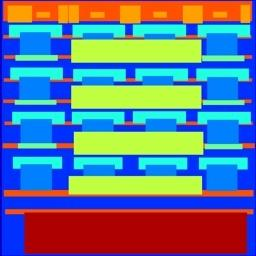
\includegraphics[width=0.2\linewidth]{figs/facades2_loss_variations_latex/input_46.jpg} &
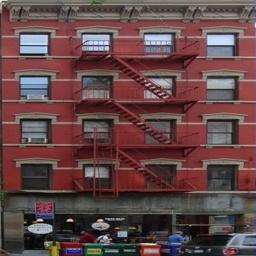
\includegraphics[width=0.2\linewidth]{figs/facades2_loss_variations_latex/gt_46.jpg} &
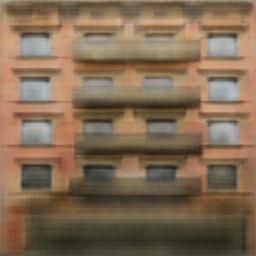
\includegraphics[width=0.2\linewidth]{figs/facades2_loss_variations_latex/L1_46.jpg} &
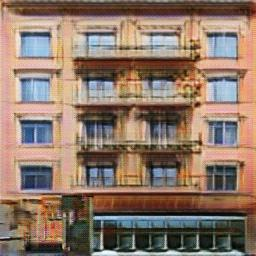
\includegraphics[width=0.2\linewidth]{figs/facades2_loss_variations_latex/cGAN_46.jpg} &
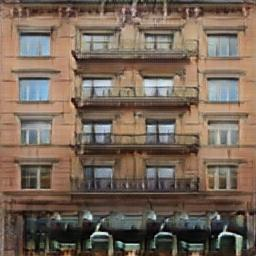
\includegraphics[width=0.2\linewidth]{figs/facades2_loss_variations_latex/L1cGAN_46.jpg} \\ 
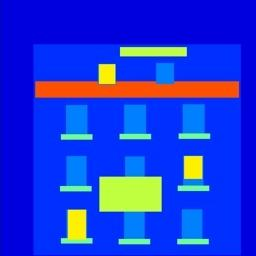
\includegraphics[width=0.2\linewidth]{figs/facades2_loss_variations_latex/input_60.jpg} &
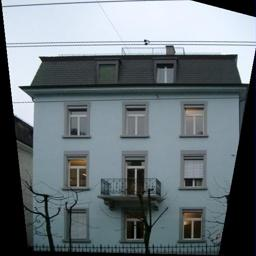
\includegraphics[width=0.2\linewidth]{figs/facades2_loss_variations_latex/gt_60.jpg} &
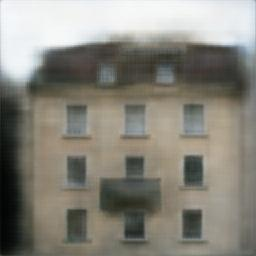
\includegraphics[width=0.2\linewidth]{figs/facades2_loss_variations_latex/L1_60.jpg} &
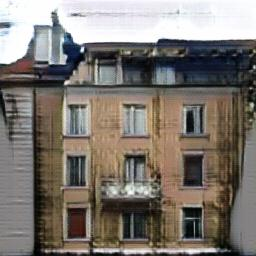
\includegraphics[width=0.2\linewidth]{figs/facades2_loss_variations_latex/cGAN_60.jpg} &
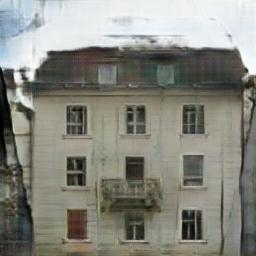
\includegraphics[width=0.2\linewidth]{figs/facades2_loss_variations_latex/L1cGAN_60.jpg}

\end{tabular} \egroup 
\end{center}
\caption{Loss variations}
\label{facades_loss_variations_qualitative}
\end{figure*}